\documentclass[journal]{IEEEtran}
\usepackage[a5paper, margin=10mm, onecolumn]{geometry}
\usepackage{lmodern} % Ensure lmodern is loaded for pdflatex
\usepackage{tfrupee} % Include tfrupee package

\setlength{\headheight}{1cm} % Set the height of the header box
\setlength{\headsep}{0mm}     % Set the distance between the header box and the top of the text

\usepackage{gvv-book}
\usepackage{gvv}
\usepackage{cite}
\usepackage{amsmath,amssymb,amsfonts,amsthm}
\usepackage{algorithmic}
\usepackage{graphicx}
\usepackage{textcomp}
\usepackage{xcolor}
\usepackage{txfonts}
\usepackage{listings}
\usepackage{enumitem}
\usepackage{mathtools}
\usepackage{gensymb}
\usepackage{comment}
\usepackage[breaklinks=true]{hyperref}
\usepackage{tkz-euclide} 
\usepackage{listings}                                      
\def\inputGnumericTable{}                                 
\usepackage[latin1]{inputenc}                                
\usepackage{color}                                            
\usepackage{array}                                            
\usepackage{longtable}
\usepackage{multicol}
\usepackage{calc}                                             
\usepackage{multirow}                                          
\usepackage{hhline}                                           
\usepackage{ifthen}                                           
\usepackage{lscape}

\begin{document}

\bibliographystyle{IEEEtran}
\vspace{3cm}

\title{11.16.3.8.3}
\author{EE24BTECH11047 - Niketh Prakash Achanta}
{\let\newpage\relax\maketitle}

\renewcommand{\thefigure}{\theenumi}
\renewcommand{\thetable}{\theenumi}
\setlength{\intextsep}{10pt} % Space between text and floats

\numberwithin{equation}{enumi}
\numberwithin{figure}{enumi}
\renewcommand{\thetable}{\theenumi}

\section{Problem Statement}
\textbf{Question}:\\
Three coins are tossed once. Find the probability of getting at least 2 heads.

\section{Solution}

\subsection{Random Variables}
Let $ X_1, X_2, X_3 $ be three independent Bernoulli random variables:
\begin{align}
X_i =
\begin{cases}
1, & \text{if Head appears,} \\
0, & \text{if Tail appears.}
\end{cases}
\end{align}
Each $X_i$ follows a Bernoulli distribution with:
\begin{align}
P_{X}(1) = p = \frac{1}{2}, \quad P_{X}(0) = 1 - p.
\end{align}

\subsection{Moment-Generating Function (MGF) Using Z-Transform}
The moment-generating function (MGF) for $X_i$ is given by:
\begin{align}
M_{X_i}\brak{z} = \sum_{k=-\infty}^{\infty} P_{X_i}\brak{k} z^{-k} = (1 - p) + pz^{-1}.
\end{align}

Using independence, the MGF of $Y = X_1 + X_2 + X_3$ is:
\begin{align}
M_Y\brak{z} = M_{X_1}\brak{z} M_{X_2}\brak{z} M_{X_3}\brak{z} = \left((1 - p) + pz^{-1}\right)^3.
\end{align}
Expanding using the binomial theorem:
\begin{align}
M_Y\brak{z} = \sum_{k=0}^{3} \binom{3}{k} (1 - p)^{3-k} p^k z^{-k}.
\end{align}
Applying the inverse Z-transform, the probability mass function (PMF) is:
\begin{align}
p_Y(k) = \binom{3}{k} (1 - p)^{3-k} p^k, \quad k = 0, 1, 2, 3.
\end{align}
Substituting $p = \frac{1}{2}$:
\begin{align}
p_Y(k) = \binom{3}{k} \left(\frac{1}{2}\right)^3.
\end{align}

\subsection{Cumulative Distribution Function (CDF)}
The cumulative distribution function (CDF) is given by:
\begin{align}
F_Y(k) = \sum_{j=-\infty}^{k} p_Y(j).
\end{align}
Substituting values:
\begin{align}
F_Y(k) =
\begin{cases}
0, & k < 0, \\
\frac{1}{8}, & 0 \leq k < 1, \\
\frac{4}{8}, & 1 \leq k < 2, \\
\frac{7}{8}, & 2 \leq k < 3, \\
1, & k \geq 3.
\end{cases}
\end{align}

\subsection{Probability of At Least Two Heads}
\begin{align}
p(Y \geq 2) = 1 - F_Y(1) = 1 - \frac{4}{8} = \frac{1}{2}.
\end{align}

\begin{figure}[!ht]
    \centering
    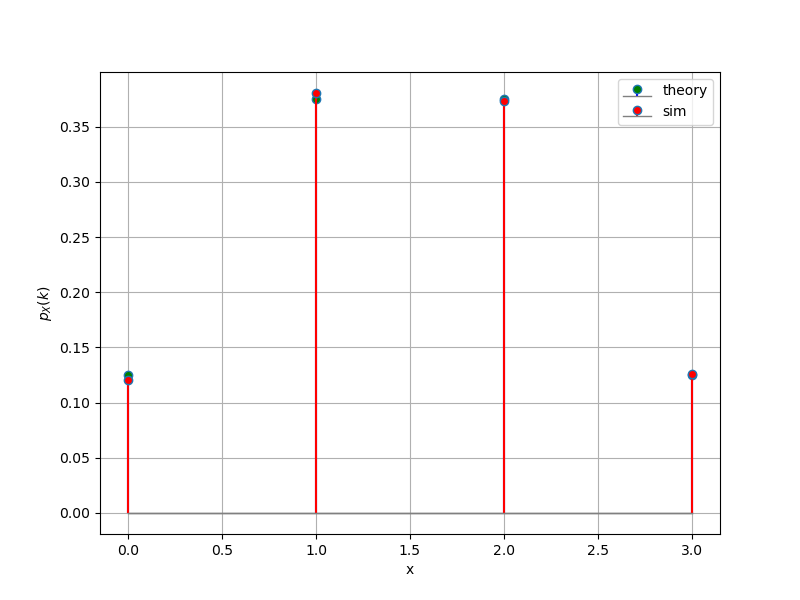
\includegraphics[width=\columnwidth]{/home/niketh/EE1003/3.8.3/figs/pmf.png}
    \caption{PMF}
\end{figure}
\begin{figure}[!ht]
    \centering
    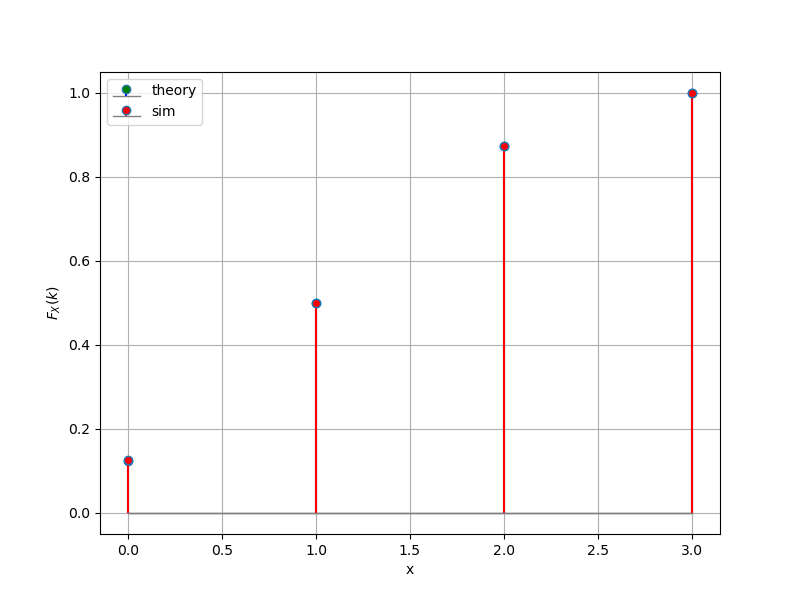
\includegraphics[width=\columnwidth]{/home/niketh/EE1003/3.8.3/figs/cdf.png}
    \caption{CDF}
\end{figure}

\end{document}

